\documentclass[12pt, letterpaper]{report}
\usepackage[margin=1in]{geometry}
\usepackage[utf8]{inputenc}
\usepackage{graphicx}
\usepackage{amsmath}
\usepackage{float}
\usepackage{subfig}
\graphicspath{ {./img/} }
\setlength\parindent{0pt}
\renewcommand{\thesection}{\Roman{section}.}
\renewcommand{\thesubsection}{\alph{subsection}.}


\title{CS1675 - Assignment 10}
\author{Zachary M. Mattis}


\begin{document}

\maketitle

\section{Problem 1 - Feature/Input Ranking}


% A
\subsection{Fisher\_score(x, y)}

\begin{table}[H]
	\centering
	\begin{tabular}{ |r|r|r| }
		\hline
		\textbf{Rank} & \textbf{Index} & \textbf{Fisher Score} \\
		\hline
		1 & 48 & 0.3192 \\
		\hline
		2 & 25 & 0.2140 \\
		\hline
		3 & 21 & 0.1910 \\
		\hline
		4 & 70 & 0.1892 \\
		\hline
		5 & 65 & 0.1693 \\
		\hline		
		6 & 40 & 0.1673 \\
		\hline
		7 & 29 & 0.1650 \\
		\hline
		8 & 19 & 0.1402 \\
		\hline
		9 & 57 & 0.1255 \\
		\hline
		10 & 20 & 0.1212 \\
		\hline
		11 & 24 & 0.0995 \\
		\hline
		12 & 30 & 0.0950 \\
		\hline
		13 & 12 & 0.0858 \\
		\hline
		14 & 47 & 0.0846 \\
		\hline
		15 & 61 & 0.0607 \\
		\hline
		16 & 10 & 0.0579 \\
		\hline
		17 & 34 & 0.0527 \\
		\hline
		18 & 27 & 0.0462 \\
		\hline
		19 & 39 & 0.0461 \\
		\hline
		20 & 41 & 0.0422 \\
		\hline
	\end{tabular}
	\caption{Fisher Score, FeatureSelectionData.txt}
\end{table}


% B
\subsection{AUROC\_score(x, y)}

\begin{table}[H]
	\centering
	\begin{tabular}{ |r|r|r| }
		\hline
		\textbf{Rank} & \textbf{Index} & \textbf{AUROC Score} \\
		\hline
		1 & 25 & 0.7340 \\
		\hline
		2 & 48 & 0.7133 \\
		\hline
		3 & 40 & 0.6887 \\
		\hline
		4 & 29 & 0.6837 \\
		\hline
		5 & 21 & 0.6833 \\
		\hline		
		6 & 67 & 0.6730 \\
		\hline
		7 & 70 & 0.6707 \\
		\hline
		8 & 11 & 0.6695 \\
		\hline
		9 & 47 & 0.6661 \\
		\hline
		10 & 65 & 0.6620 \\
		\hline
		11 & 12 & 0.6459 \\
		\hline
		12 & 24 & 0.6432 \\
		\hline
		13 & 39 & 0.6412 \\
		\hline
		14 & 6 & 0.6383 \\
		\hline
		15 & 19 & 0.6315 \\
		\hline
		16 & 57 & 0.6270 \\
		\hline
		17 & 20 & 0.6280 \\
		\hline
		18 & 34 & 0.6174 \\
		\hline
		19 & 5 & 0.6168 \\
		\hline
		20 & 14 & 0.6090 \\
		\hline
	\end{tabular}
	\caption{AUROC Score, FeatureSelectionData.txt}
\end{table}


There are a total of 15 shared dimensions between the two result sets. They are not in the same order, but they are relatively close. This is expected as the dimensions that have the greatest predictive power should be very similar across different interpretative algorithms.


\section{Problem 2 - Bagging of Classifiers}

% A
\subsection{Bagging}

\begin{table}[H]
	\centering
	\begin{tabular}{ |r|r|r| }
		\hline
		\textbf{T} & \textbf{Training} & \textbf{Testing} \\
		\hline
		1 & 0.1046 & 0.2164 \\
		\hline
		2 & 0.0900 & 0.1486 \\
		\hline
		3 & 0.0558 & 0.1657 \\
		\hline
		4 & 0.0523 & 0.1443 \\
		\hline
		5 & 0.0369 & 0.1643 \\
		\hline
		6 & 0.0342 & 0.1236 \\
		\hline
		7 & 0.0258 & 0.1507 \\
		\hline
		8 & 0.0242 & 0.1357 \\
		\hline
		9 & 0.0200 & 0.1429 \\
		\hline
		10 & 0.0181 & 0.1393 \\
		\hline
	\end{tabular}
	\caption{Bagging SVM}
\end{table}


\begin{figure}[H]
	\centering
	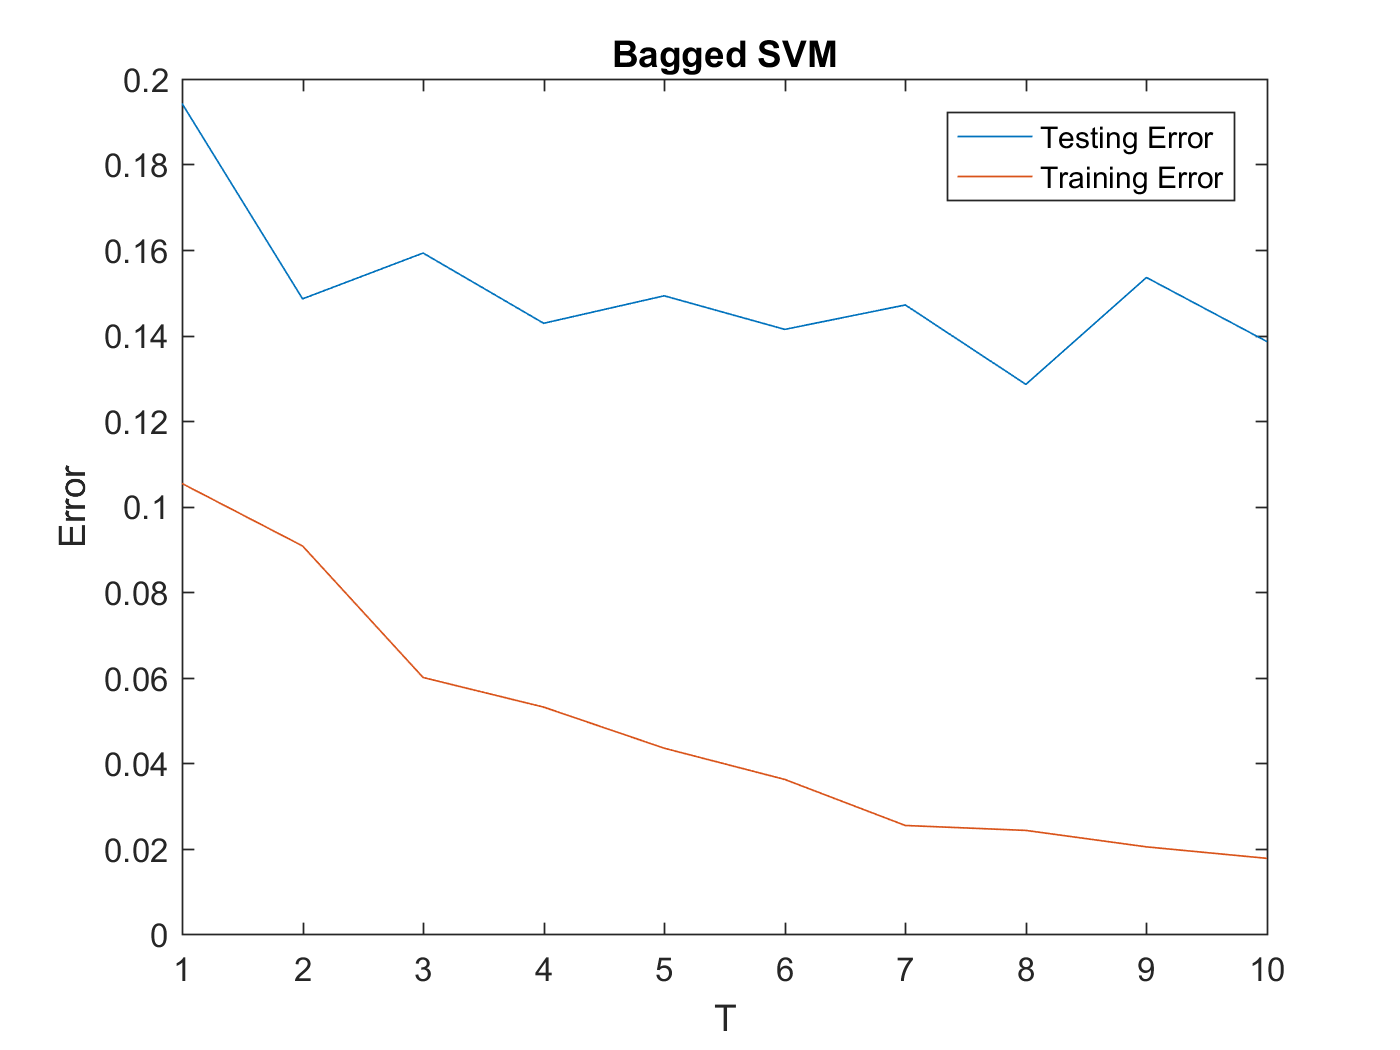
\includegraphics[width=0.7\columnwidth]{bag_svm.png}
	\caption{Bagged SVM}
\end{figure}


An observation of the bagged SVM plot demonstrates a steady decreasing of the training error as the number of models increases. However, the testing error appears to approach a constant of $\sim 0.14$.


% B
\subsection{Decision Tree}


\begin{table}[H]
	\centering
	\begin{tabular}{ |r|r|r| }
		\hline
		\textbf{T} & \textbf{Training} & \textbf{Testing} \\
		\hline
		1 & 0.1396 & 0.2521 \\
		\hline
		2 & 0.1235 & 0.1771 \\
		\hline
		3 & 0.0781 & 0.2243 \\
		\hline
		4 & 0.0723 & 0.1543 \\
		\hline
		5 & 0.0423 & 0.1886 \\
		\hline
		6 & 0.0546 & 0.1443 \\
		\hline
		7 & 0.0292 & 0.1671 \\
		\hline
		8 & 0.0365 & 0.1464 \\
		\hline
		9 & 0.0200 & 0.1443 \\
		\hline
		10 & 0.0335 & 0.1343 \\
		\hline
	\end{tabular}
	\caption{Decision Tree}
\end{table}


\begin{figure}[H]
	\centering
	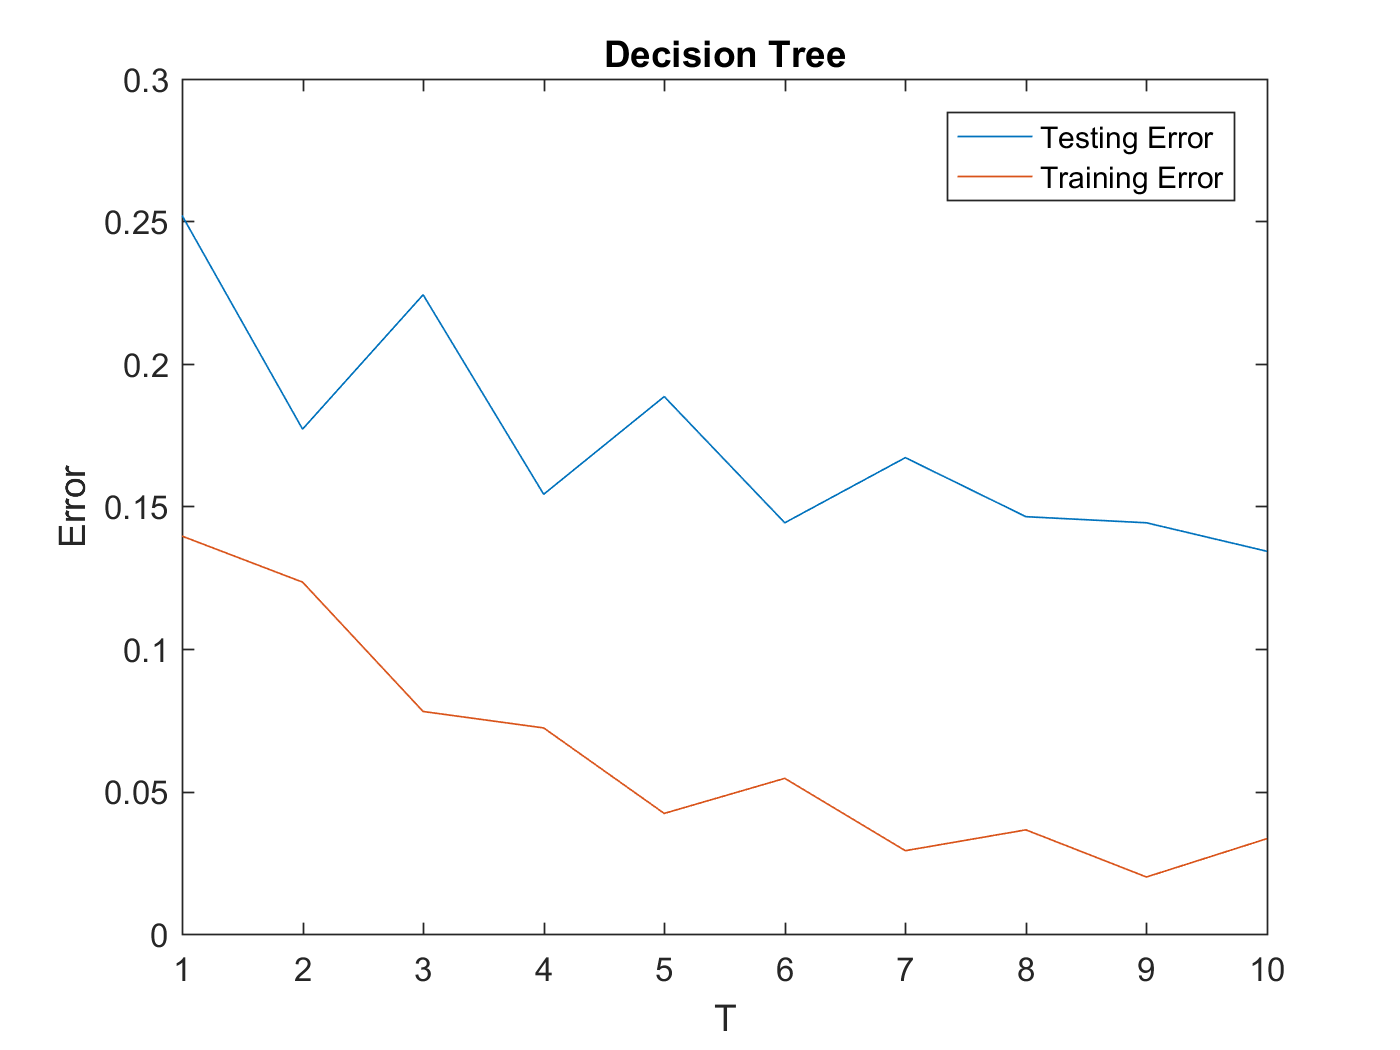
\includegraphics[width=0.7\columnwidth]{decision_tree.png}
	\caption{Decision Tree}
\end{figure}


An observation of the Decision Tree plot yields similar results to the bagging SVM above. This graph demonstrates a generally steady decreasing of the training error as the number of models increases. However, the testing error appears to approach a constant of $\sim 0.14$.


\end{document}